% !TEX root = ../../autoreferat.tex
\section{Vytvoření řečového korpusu EL promluv}
\label{chap:construction:corpus}

% Před započetím prací na vytvoření ASR systému pracujícího s~lidmi po TL je potřeba vytvořit řečový korpus, který poslouží  k~natrénování a otestování vytvořeného systému. Tato data jsou velmi specifická. Proto je potřeba zajistit co možná největší množství kvalitních\footnote{Kvalitou je myšlena věrnost dat dané doméně, dále se mluví o přesnosti ve smyslu bezchybnosti přepisů.} a přesných dat, která budou součástí řečového korpusu.

% Jak už bylo zmíněno v~části \ref{chap:cause:desease}, ročně se objeví více než 100 nových případů trvalé ztráty hlasu, přičemž rizikovou skupinou osob jsou starší lidé, kteří intenzivně kouří a konzumují alkohol. Přesto je patrný trend snižujícího se věku pacientů a s~tím související nárůst případů ztráty hlasu. Přičteme-li již výše zmíněný psychologický aspekt jeho ztráty, je zřejmé, jak komplikované je zajistit spolupráci byť s~jediným řečníkem ochotným podstoupit náročné\footnote{I pro zdravého člověka je někdy několikahodinové nahrávání vysilující. Pro jedince po TL to je z mnoha důvodů ještě řádově náročnější.} nahrávání.

% Proto došlo  k~navázání kontaktů se specializovanými pracovišti ORL, v~našem případě byly nejprve navázány kontakty s~ORL klinikou při Fakultní nemocnici v~Plzni, a následně i s~ORL klinikou Fakultní nemocnice v~Motole.
S pomocí lékařů ORL kliniky při Fakultní nemocnici v~Plzni byla navázána spolupráce s~jedním řečníkem, konkrétně se jedná o dámu v~důchodovém věku, která podstoupila TL před více než 15 lety.
% Po překonání ostychu\footnote{Podle jejích vlastních slov nebyla schopna několik let po operaci ani zvednout nečekaný telefonní hovor, natož mluvit na veřejnosti.} se byla schopna naplno vrátit do běžného života a dokonce v~určité formě opět přednášet o stomatologii na Lékařské fakultě v~Plzni, Univerzity Karlovy.
S její pomocí bylo na pracovišti Katedry kybernetiky ZČU v~1.~etapě nahrávání,
% v~období od prosince 2010 do května 2011,
pořízeno více než 10 hodin promluv.
% během 14 samostatných sezení více než 10 hodin promluv, viz tab. \ref{tab:construction:recording}.
% Každé sezení trvalo přibližně dvě hodiny a bylo rozděleno na fáze nahrávání a fáze odpočinku. Fáze nahrávání trvaly 10 - 20 minut.
Pořízené dílčí nahrávky obsahují několik vět, které jsou vzájemně odděleny úseky ticha o minimální délce 5~s.
% Fáze odpočinku mezi nahráváním dílčích segmentů trvaly přibližně 10 minut.
% Bylo nezbytné je do harmonogramu zařadit zejména z~důvodu únavy řečníka.
Získaná data neobsahují žádný nežádoucí ruch kromě samotného zvuku EL i přesto, že nahrávání neprobíhalo v~profesionálním studiu.

% \begin{table}[htpb]
%   \centering
%   \def\arraystretch{1.5}
%   \pgfplotstabletypeset[
%     col sep=comma,
%     string type,
%     columns/phase/.style={column name={Nahrávání}, column type={l}},
%     columns/length/.style={column name={Délka \textit{[HH:MM:SS]}}, column type={r}},
%     columns/sentences/.style={column name={Počet vět}, column type={r}},
%     columns/files/.style={column name={Počet souborů}, column type={r}},
%     every head row/.style={
%       after row={
%         \cmidrule(r){1-1}
%         \cmidrule(lr){2-2}
%         \cmidrule(lr){3-3}
%         \cmidrule(l){4-4}
%       },
%       before row={\toprule}
%     },
%     every last row/.style={after row={\bottomrule}},
%   ]{./parts/ch5-construction/tabs/02-recording1-stats.csv}
%   \caption{Informace o korpusu nahrávek z 1. etapy nahrávání.}
%   \label{tab:construction:recording}
% \end{table}

Pro pořízení záznamů byla navržena nahrávací sestava složená z miniaturního profesionálního mikrofonu (DPA d:screet 4061-FM), zesilovače (DPA MMA6000), externí zvukové karty a běžného notebooku. Mikrofon byl pomocí bezpolštářkové náplasti přilepen co nejblíže (do bezprostřední blízkosti) pravého koutku úst mluvčí tak, aby zaznamenaná řeč měla co možná nejvyšší kvalitu.

Před samotným nahrávánám byly z databáze obsahující stovky tisíc vět pečlivě vybrány, postupem popsaným v~\cite{Radova2000}, konkrétní věty a z nich vytvořeny 2 sady vět, konkrétně:

\begin{enumerate}
  \item sada obsahující všechny fonémy vyskytující se v~češtině - \textit{40 vět};
  \item sada obsahující věty s~reálnou četností fonémů - \textit{5000 vět}.
\end{enumerate}

% \noindent Nahrané soubory vždy obsahují několik vět vzájemně oddělených minimálně 5 sekundovými úseky ticha.
% Nahrávky mouhou navíc obsahovat opakování chybně vyslovených vět, přeřeknutí, kýchnutí a další neřečové události.
% Z tohoto důvodu bylo nezbytné nahrávky rozčlenit na kratší úseky a anotovat, přestože byly pořízené na základě připravené sady vět.

Každá nahrávka je automaticky rozdělena na mikrosegmenty o konzistentní době trvání. Empiricky byla stanovena vhodná délka trvání v~rozsahu 10 - 100 ms. S~využitím metody voice activity detection (VAD) byla pro každou nahrávku stanovena hodnota energie dle vztahu

\begin{equation}
  \label{eq:construction:energy}
  E_{RMS}(n) = \sqrt{\frac{1}{N} \sum_{n=1}^{N} \left| x(n) \right|^2},
\end{equation}

\noindent kde $N$ představuje počet vzorků v~nahrávce a $x(n)$ představuje pravoúhlé okénko vzorku $n$ a následně určena průměrná energie nahrávky jako střední hodnota energií všech mikrosegmentů.
Její hodnota slouží pro nalezení úseků ticha, tj. míst, kde začíná a končí věta.
Pokud energie nějakého úseku $x$ je $E_{RMS}(x) < avg(E_{RMS})$ a zároveň délka tohoto úseku $dur(x) \geq 1\ s$, tak je možné nahrávku v~tomto úseku rozdělit.
% Na začátku a konci každého úseku je vhodné mít minimálně $0.5\ s$ ticha, aby byla zajištěna správná funkce ASR systému, viz \ref{chap:asr:parametrization}.
Na obr. \ref{fig:construction:el_speech} je zobrazena ukázka charakteru audio signálu a spektrogram promluvy \textit{\uv{Akcie Komerční banky}}.
% Zároveň jsou zde vyneseny vypočtené hodnoty energie a celková průměrná energie.
% Pokud řečník v~průběhu věty z~libovolného důvodu udělal pauzu větší než $1\ s$, tak i tato věta byla v~důsledku výše popsaného postupu rozdělena na dvě části.
% Nejedná se však o významný problém, protože při vytváření ASR systému není podstatné, zda promluva představuje celou větu, ale spíše to, zda je tento úsek správně přepsán.
% Fakt, že některé věty jsou rozděleny na více částí, je důvodem, proč v~tab. \ref{tab:construction:recording} neodpovídá počet soubourů počtu vět.

\begin{figure}[hbpt]
  \centering
  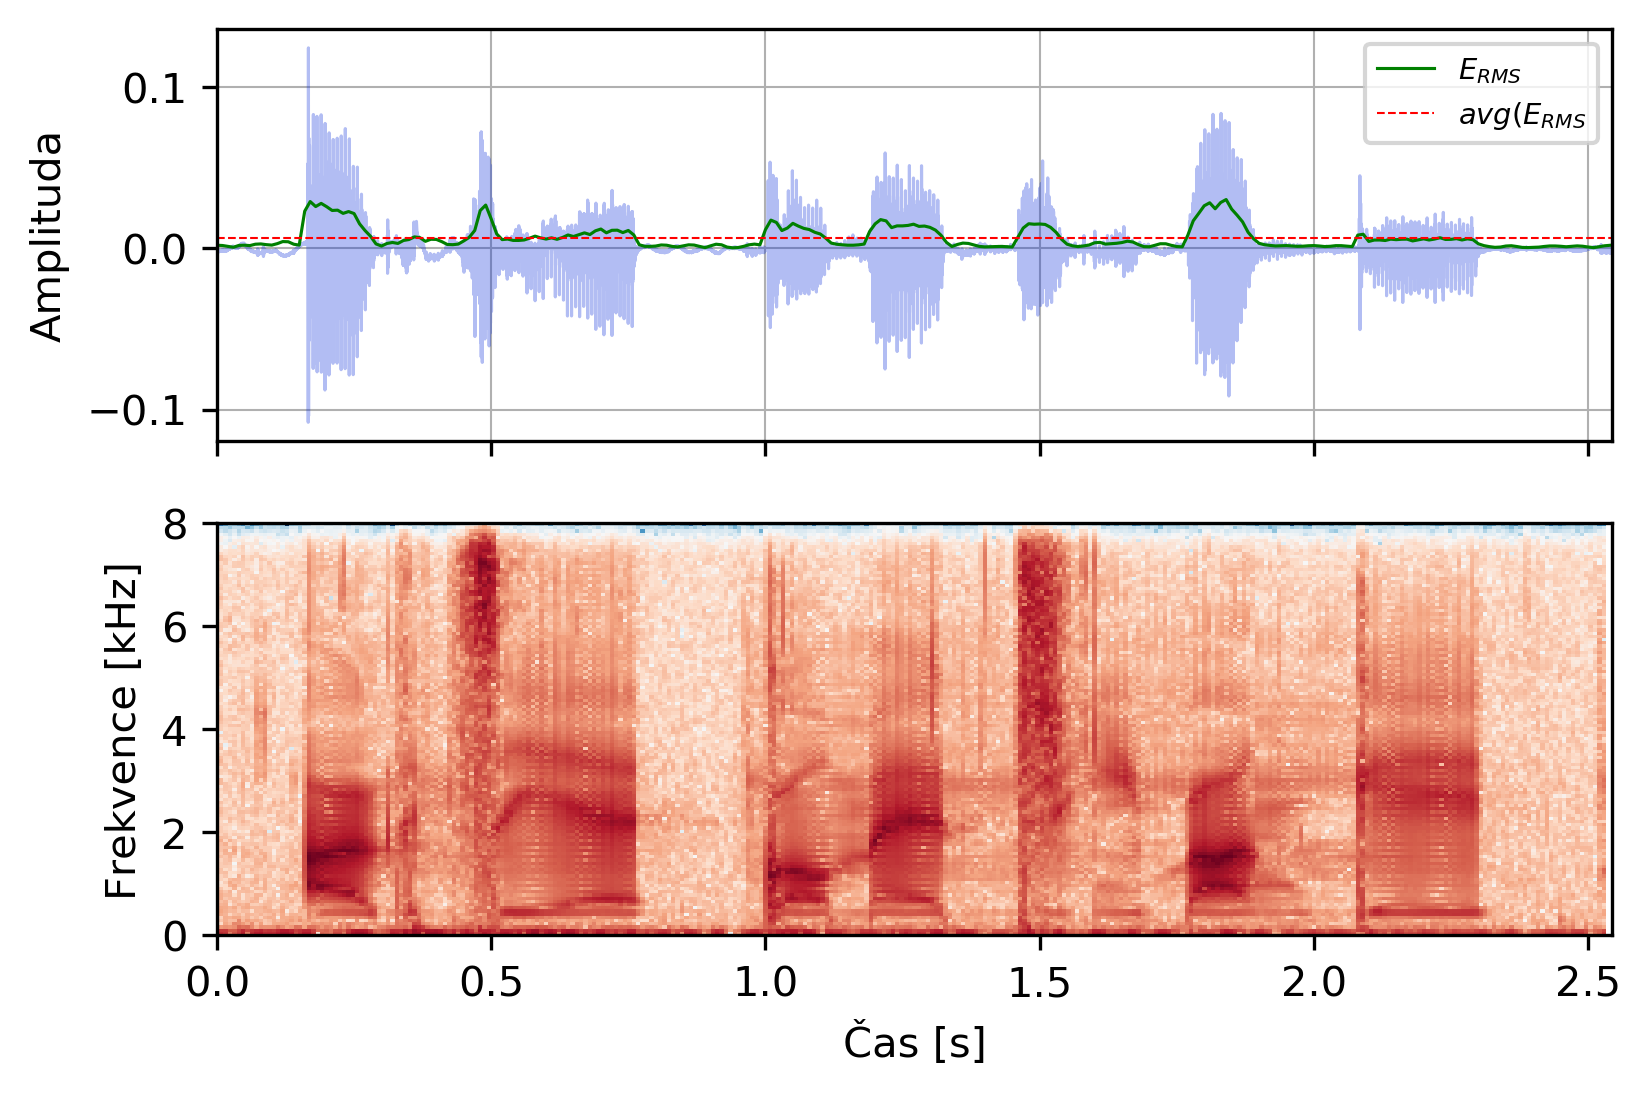
\includegraphics[width=0.9\textwidth]{./parts/ch5-construction/img/energy_spec_el.png}
  \caption[Průběh a spektrogram EL promluvy.]{Průběh a spektrogram promluvy a vyznačenou energií EL promluvy.}
  \label{fig:construction:el_speech}
\end{figure}

% K anotaci posloužil interní anotační nástroj, podíleli se na ní celkem 3 anotátoři z~řad studentů.
% Přepis každého anotátora byl vždy zkontrolován jiným anotátorem.
% Ačkoli bylo potřeba přepsat relativně malé množství dat (cca 10 hodin audio záznamu), tak anotace všech promluv trvala přibližně 2 měsíce.
% Hlavním důvodem byla relativně dlouhá doba, po kterou se anotátoři adaptovali na specifika EL řeči.
% Hlavně ze začátku nebyli schopni porozumět obsahu promluvy, a tím pádem jej správně přepsat.
% To významně prodloužilo dobu potřebnou  k~anotaci celého řečového korpusu.

% Pokud je  k~produkci řeči použit elektrolarynx, je vedlejším produktem nezanedbatelný ruch způsobený samotným zařízením, viz část \ref{chap:cause:treatment:foniatric}.
% Z~tohoto důvodu byly v~průběhu anotace ignorovány v~podstatě všechny skupiny neřečových událostí, protože vetšina nahrávek by dle pravidel anotování běžné řeči obsahovala šum.
% Výsledný řečový korpus se skládá z $5040$ unikátních vět rozdělených do $6385$ souborů (viz tab. \ref{tab:construction:recording}), které v~průměru obsahují $7$ slov o průměrné délce $5$ znaků. Tento korpus slouží jako základ pro všechny budoucí experimenty.
